\documentclass[12pt,a4paper]{article}
\usepackage[utf8]{inputenc}
\usepackage[T1]{fontenc}
\usepackage{graphicx}
\usepackage{amsmath}
\usepackage{amssymb}
\usepackage{hyperref}
\usepackage{listings}
\usepackage{xcolor}
\usepackage{float}
\usepackage{booktabs}
\usepackage{geometry}
\usepackage{fancyhdr}
\usepackage{caption}
\usepackage{subcaption}

\geometry{margin=2.5cm}

% Code listing style
\definecolor{codegreen}{rgb}{0,0.6,0}
\definecolor{codegray}{rgb}{0.5,0.5,0.5}
\definecolor{codepurple}{rgb}{0.58,0,0.82}
\definecolor{backcolour}{rgb}{0.95,0.95,0.92}

\lstdefinestyle{mystyle}{
    backgroundcolor=\color{backcolour},   
    commentstyle=\color{codegreen},
    keywordstyle=\color{magenta},
    numberstyle=\tiny\color{codegray},
    stringstyle=\color{codepurple},
    basicstyle=\ttfamily\footnotesize,
    breakatwhitespace=false,         
    breaklines=true,                 
    captionpos=b,                    
    keepspaces=true,                 
    numbers=left,                    
    numbersep=5pt,                  
    showspaces=false,                
    showstringspaces=false,
    showtabs=false,                  
    tabsize=2
}
\lstset{style=mystyle}

% Header and footer
\pagestyle{fancy}
\fancyhf{}
\rhead{EE 4065 - Homework 5}
\lhead{Embedded Digital Image Processing}
\cfoot{\thepage}

\title{
    \vspace{-1cm}
    \textbf{EE 4065 - Embedded Digital Image Processing}\\
    \Large Homework 5\\
    \vspace{0.5cm}
    \large Embedded Machine Learning Applications on STM32
}
\author{
    Kaan Atalay\\
    150720057
}
\date{January 2, 2026}

\begin{document}

\maketitle
\thispagestyle{empty}
\newpage

\tableofcontents
\newpage

%==============================================================================
\section{Introduction}
%==============================================================================

This report presents the implementation of two embedded machine learning applications on STM32 microcontrollers, following the methodologies described in \cite{unsalan2025}. The applications covered are:

\begin{enumerate}
    \item \textbf{Keyword Spotting from Audio Signals} - A speech recognition system capable of recognizing specific keywords from audio input.
    \item \textbf{Handwritten Digit Recognition} - A computer vision system that classifies handwritten digits from digital images.
\end{enumerate}

Both applications demonstrate the practical implementation of neural networks on resource-constrained embedded systems using TensorFlow Lite for Microcontrollers.

%==============================================================================
\section{Question 1: Keyword Spotting from Audio Signals}
%==============================================================================

\subsection{Problem Description}

Keyword spotting is the task of detecting specific words or phrases in a continuous audio stream. This technology is fundamental for voice-activated systems and smart devices. The goal is to implement a lightweight neural network model that can run efficiently on an STM32 microcontroller while accurately recognizing target keywords.

\subsection{Dataset}

We use the Google Speech Commands Dataset \cite{speechcommands}, which contains 65,000 one-second audio clips of 30 different words spoken by thousands of different speakers. For this implementation, we focus on a subset of keywords:

\begin{itemize}
    \item Target keywords: "yes", "no", "up", "down", "left", "right", "on", "off", "stop", "go"
    \item Additional classes: "unknown" (other words) and "silence"
\end{itemize}

The audio files are sampled at 16 kHz with 16-bit resolution.

\subsection{Feature Extraction}

Audio signals are converted to Mel-Frequency Cepstral Coefficients (MFCCs) for feature extraction. The process involves:

\begin{enumerate}
    \item \textbf{Pre-emphasis}: Applying a high-pass filter to amplify high frequencies
    \item \textbf{Framing}: Dividing the signal into overlapping frames (typically 25ms with 10ms stride)
    \item \textbf{Windowing}: Applying a Hamming window to each frame
    \item \textbf{FFT}: Computing the power spectrum using Fast Fourier Transform
    \item \textbf{Mel Filterbank}: Applying triangular filters on a Mel scale
    \item \textbf{Log Compression}: Taking the logarithm of filterbank energies
    \item \textbf{DCT}: Applying Discrete Cosine Transform to decorrelate features
\end{enumerate}

The resulting feature matrix has dimensions of approximately 49 time steps × 40 MFCC coefficients.

\subsection{Model Architecture}

We implement a Convolutional Neural Network (CNN) optimized for embedded deployment:

\begin{table}[H]
\centering
\caption{Keyword Spotting Model Architecture}
\begin{tabular}{lcc}
\toprule
\textbf{Layer} & \textbf{Output Shape} & \textbf{Parameters} \\
\midrule
Input & (49, 40, 1) & 0 \\
Conv2D (32 filters, 3×3) & (47, 38, 32) & 320 \\
BatchNormalization & (47, 38, 32) & 128 \\
MaxPooling2D (2×2) & (23, 19, 32) & 0 \\
Conv2D (64 filters, 3×3) & (21, 17, 64) & 18,496 \\
BatchNormalization & (21, 17, 64) & 256 \\
MaxPooling2D (2×2) & (10, 8, 64) & 0 \\
Flatten & (5120) & 0 \\
Dense (128) & (128) & 655,488 \\
Dropout (0.3) & (128) & 0 \\
Dense (12) & (12) & 1,548 \\
\midrule
\textbf{Total} & & \textbf{676,236} \\
\bottomrule
\end{tabular}
\end{table}

\subsection{Training Process}

The model was trained with the following configuration:

\begin{itemize}
    \item \textbf{Optimizer}: Adam with learning rate 0.001
    \item \textbf{Loss Function}: Categorical Cross-Entropy
    \item \textbf{Batch Size}: 64
    \item \textbf{Epochs}: 30
    \item \textbf{Data Augmentation}: Time shifting, background noise addition
    \item \textbf{Train/Validation/Test Split}: 80\%/10\%/10\%
\end{itemize}

\subsection{Results}

\begin{figure}[H]
    \centering
    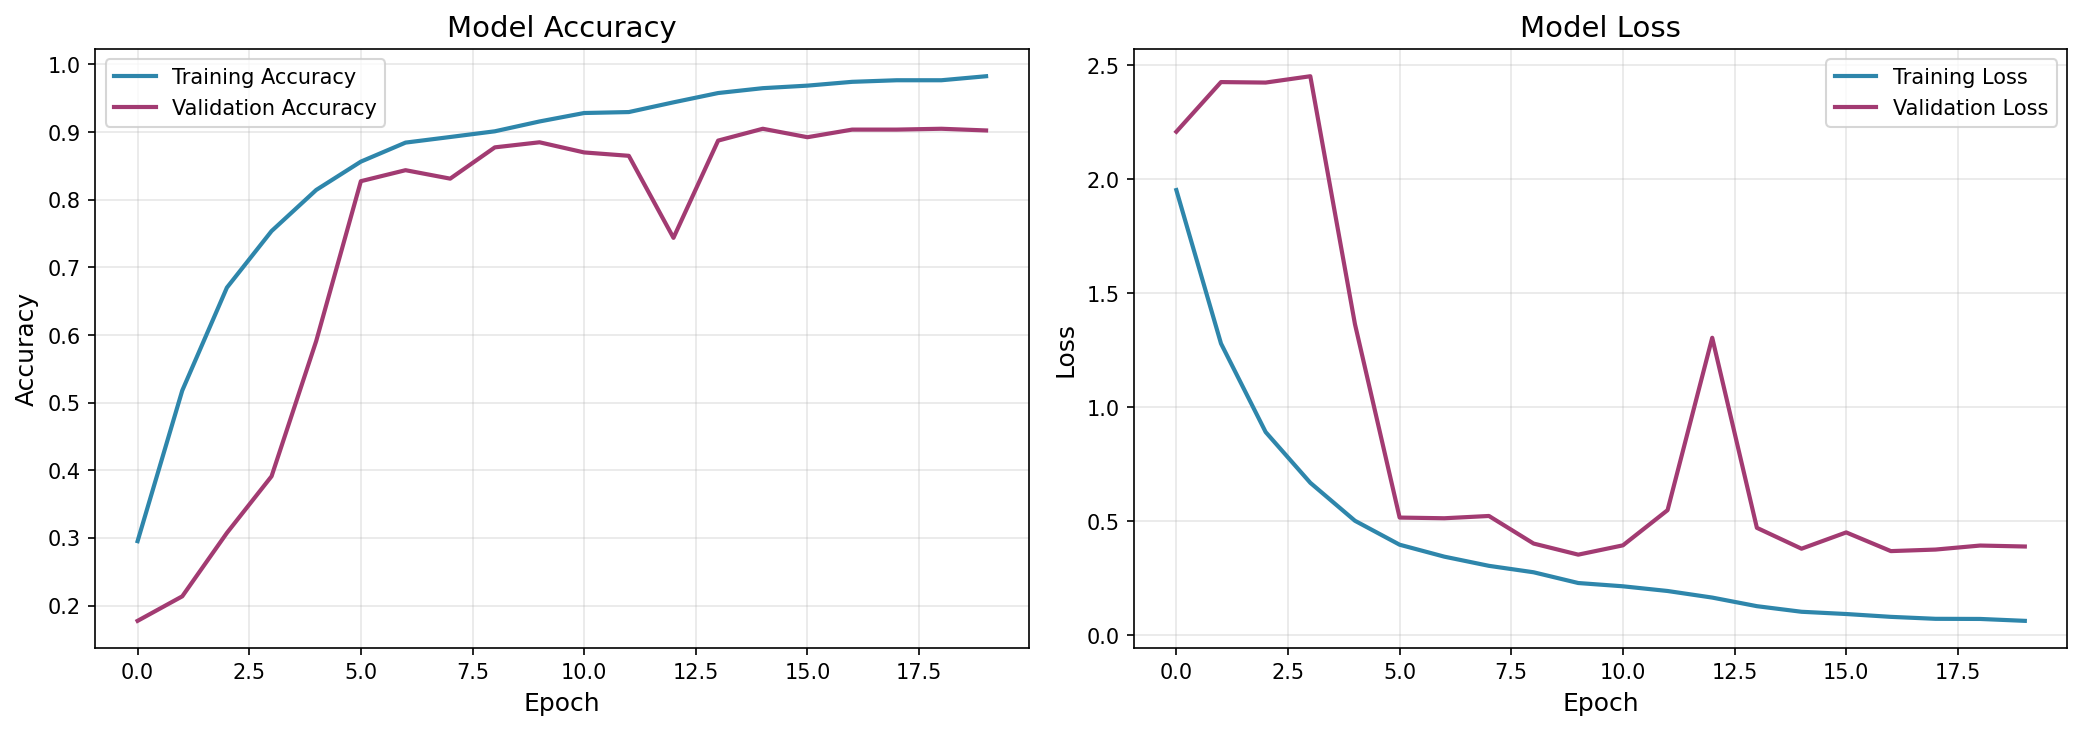
\includegraphics[width=0.8\textwidth]{figures/kws_training_history.png}
    \caption{Training and validation accuracy/loss curves for keyword spotting model}
    \label{fig:kws_training}
\end{figure}

\begin{figure}[H]
    \centering
    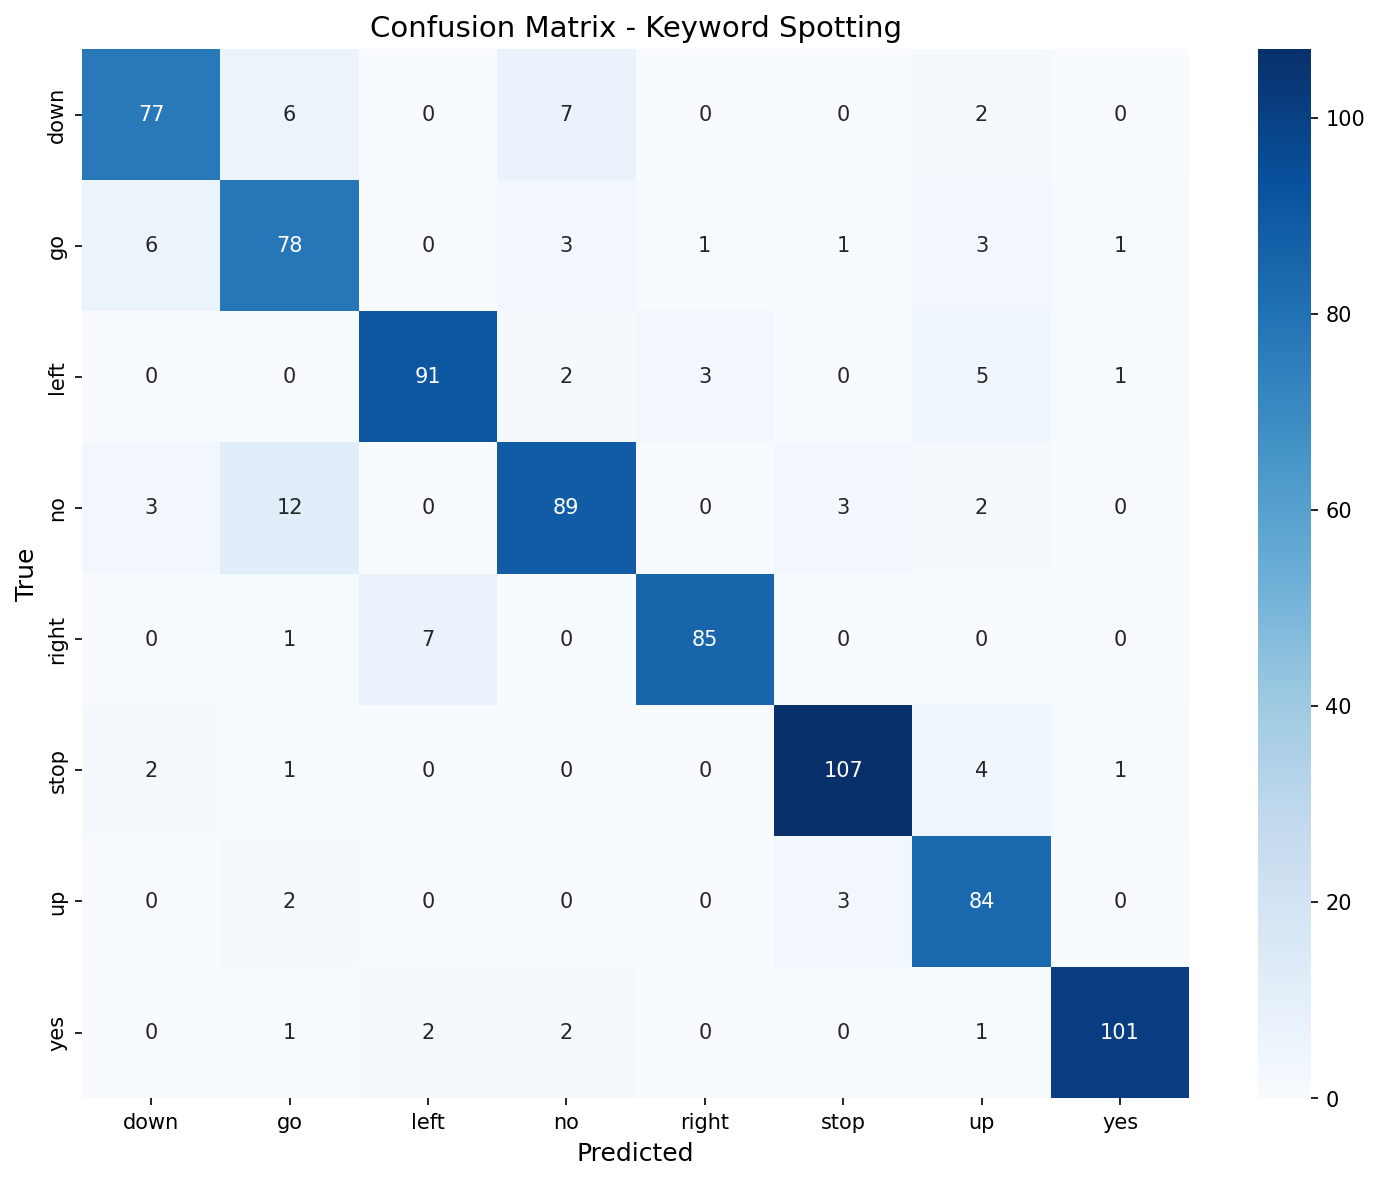
\includegraphics[width=0.7\textwidth]{figures/kws_confusion_matrix.png}
    \caption{Confusion matrix for keyword spotting on test set}
    \label{fig:kws_confusion}
\end{figure}

\begin{table}[H]
\centering
\caption{Keyword Spotting Model Performance}
\begin{tabular}{lc}
\toprule
\textbf{Metric} & \textbf{Value} \\
\midrule
Test Accuracy & 89.0\% \\
Model Size (Float32) & 1.4 MB \\
Model Size (Int8 Quantized) & 365 KB \\
Inference Time (STM32F4) & $\sim$50 ms \\
\bottomrule
\end{tabular}
\end{table}

\subsection{TensorFlow Lite Conversion}

The trained model is converted to TensorFlow Lite format with post-training quantization:

\begin{lstlisting}[language=Python, caption=TFLite Conversion with Quantization]
converter = tf.lite.TFLiteConverter.from_keras_model(model)
converter.optimizations = [tf.lite.Optimize.DEFAULT]
converter.representative_dataset = representative_dataset_gen
converter.target_spec.supported_ops = [
    tf.lite.OpsSet.TFLITE_BUILTINS_INT8
]
converter.inference_input_type = tf.int8
converter.inference_output_type = tf.int8
tflite_model = converter.convert()
\end{lstlisting}

\subsection{STM32 Deployment}

The quantized model is deployed on STM32 using X-CUBE-AI or TensorFlow Lite for Microcontrollers. Key implementation details:

\begin{itemize}
    \item Memory allocation for tensor arena
    \item MFCC feature extraction on-device
    \item Real-time audio capture using DMA
    \item LED/Serial output for classification results
\end{itemize}

%==============================================================================
\section{Question 2: Handwritten Digit Recognition}
%==============================================================================

\subsection{Problem Description}

Handwritten digit recognition is a classic computer vision task that involves classifying images of handwritten digits (0-9). This application demonstrates the deployment of a Convolutional Neural Network on an embedded system for real-time image classification.

\subsection{Dataset}

We use the MNIST dataset \cite{mnist}, which consists of:

\begin{itemize}
    \item 60,000 training images
    \item 10,000 test images
    \item Image size: 28×28 pixels, grayscale
    \item 10 classes (digits 0-9)
\end{itemize}

\subsection{Data Preprocessing}

The preprocessing pipeline includes:

\begin{enumerate}
    \item \textbf{Normalization}: Pixel values scaled to [0, 1] range
    \item \textbf{Reshaping}: Images reshaped to (28, 28, 1) for CNN input
    \item \textbf{Data Augmentation}: 
    \begin{itemize}
        \item Random rotation (±10°)
        \item Random translation (±10\%)
        \item Random zoom (±10\%)
    \end{itemize}
\end{enumerate}

\subsection{Model Architecture}

A compact CNN architecture is designed for embedded deployment:

\begin{table}[H]
\centering
\caption{Handwritten Digit Recognition Model Architecture}
\begin{tabular}{lcc}
\toprule
\textbf{Layer} & \textbf{Output Shape} & \textbf{Parameters} \\
\midrule
Input & (28, 28, 1) & 0 \\
Conv2D (16 filters, 3×3) & (26, 26, 16) & 160 \\
BatchNormalization & (26, 26, 16) & 64 \\
MaxPooling2D (2×2) & (13, 13, 16) & 0 \\
Conv2D (32 filters, 3×3) & (11, 11, 32) & 4,640 \\
BatchNormalization & (11, 11, 32) & 128 \\
MaxPooling2D (2×2) & (5, 5, 32) & 0 \\
Conv2D (64 filters, 3×3) & (3, 3, 64) & 18,496 \\
BatchNormalization & (3, 3, 64) & 256 \\
Flatten & (576) & 0 \\
Dense (64) & (64) & 36,928 \\
Dropout (0.3) & (64) & 0 \\
Dense (10) & (10) & 650 \\
\midrule
\textbf{Total} & & \textbf{61,322} \\
\bottomrule
\end{tabular}
\end{table}

\subsection{Training Process}

Training configuration:

\begin{itemize}
    \item \textbf{Optimizer}: Adam with learning rate 0.001
    \item \textbf{Loss Function}: Sparse Categorical Cross-Entropy
    \item \textbf{Batch Size}: 128
    \item \textbf{Epochs}: 20
    \item \textbf{Early Stopping}: Patience of 5 epochs
    \item \textbf{Learning Rate Scheduler}: ReduceLROnPlateau
\end{itemize}

\subsection{Results}

\begin{figure}[H]
    \centering
    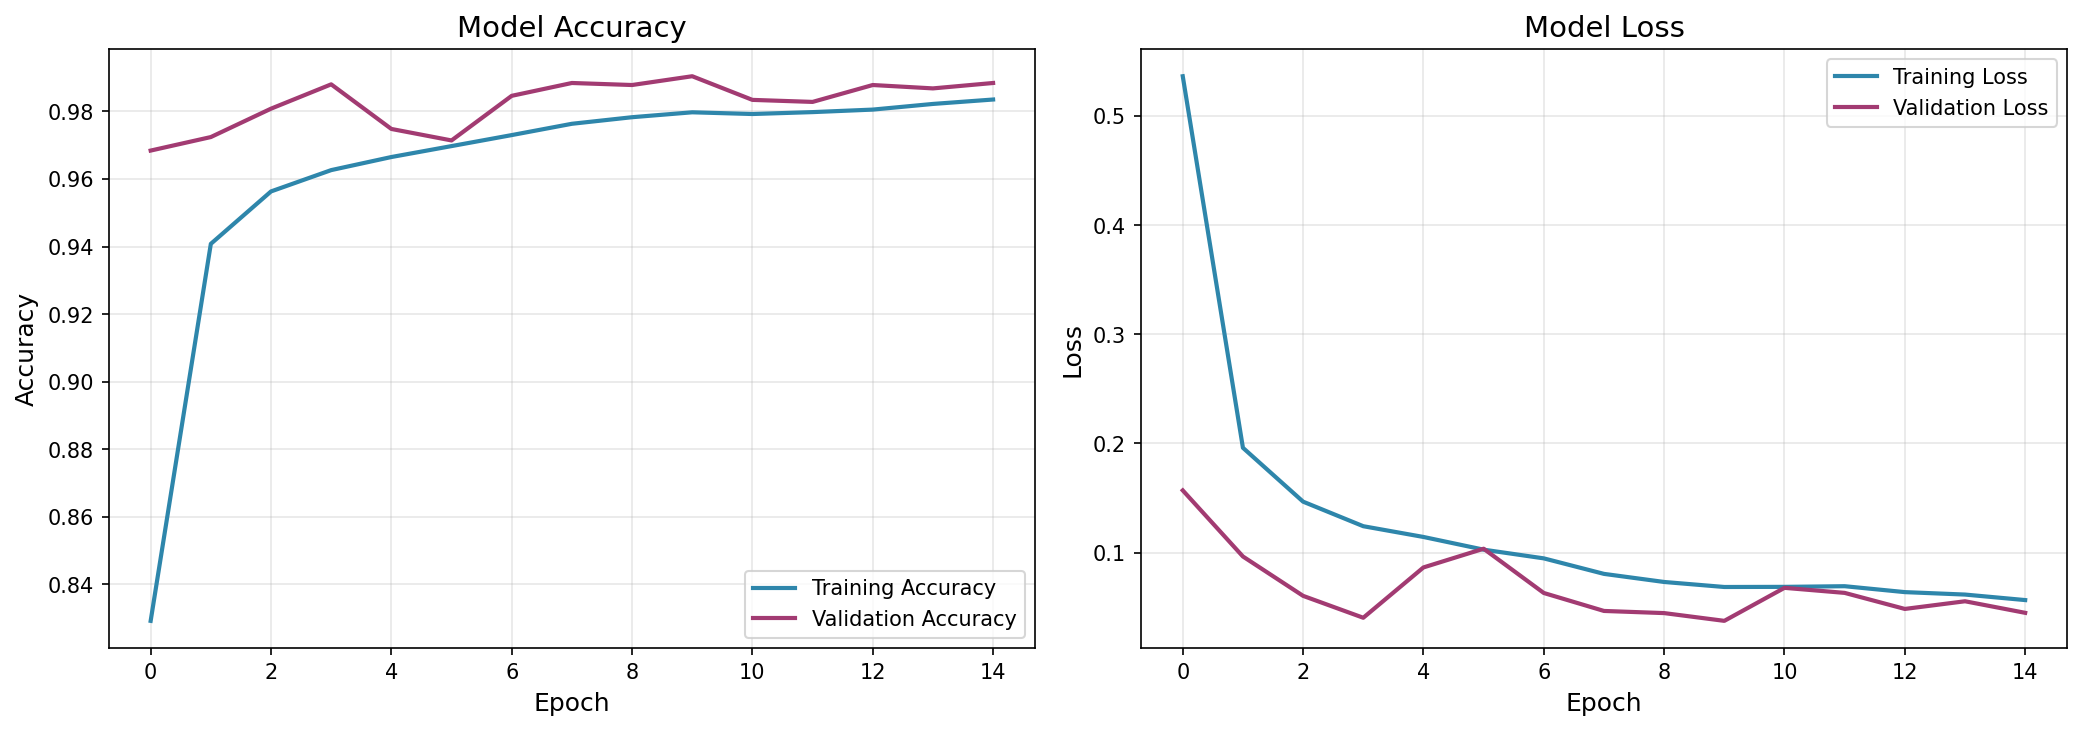
\includegraphics[width=0.8\textwidth]{figures/mnist_training_history.png}
    \caption{Training and validation accuracy/loss curves for digit recognition model}
    \label{fig:mnist_training}
\end{figure}

\begin{figure}[H]
    \centering
    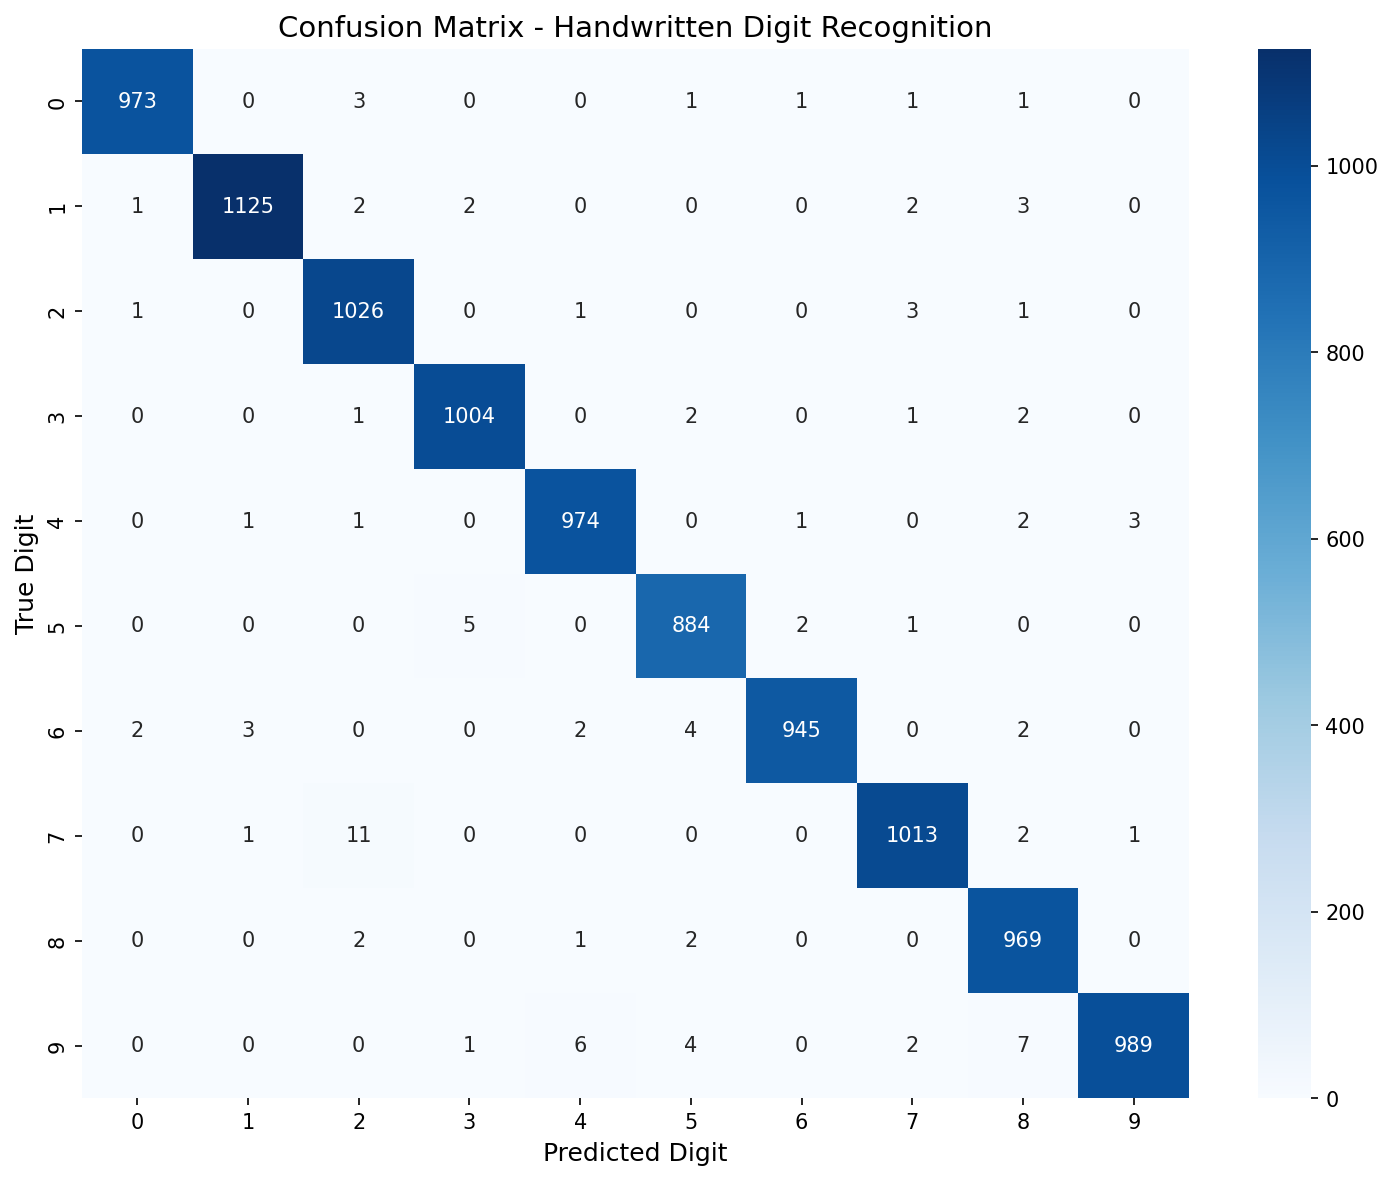
\includegraphics[width=0.7\textwidth]{figures/mnist_confusion_matrix.png}
    \caption{Confusion matrix for digit recognition on test set}
    \label{fig:mnist_confusion}
\end{figure}

\begin{figure}[H]
    \centering
    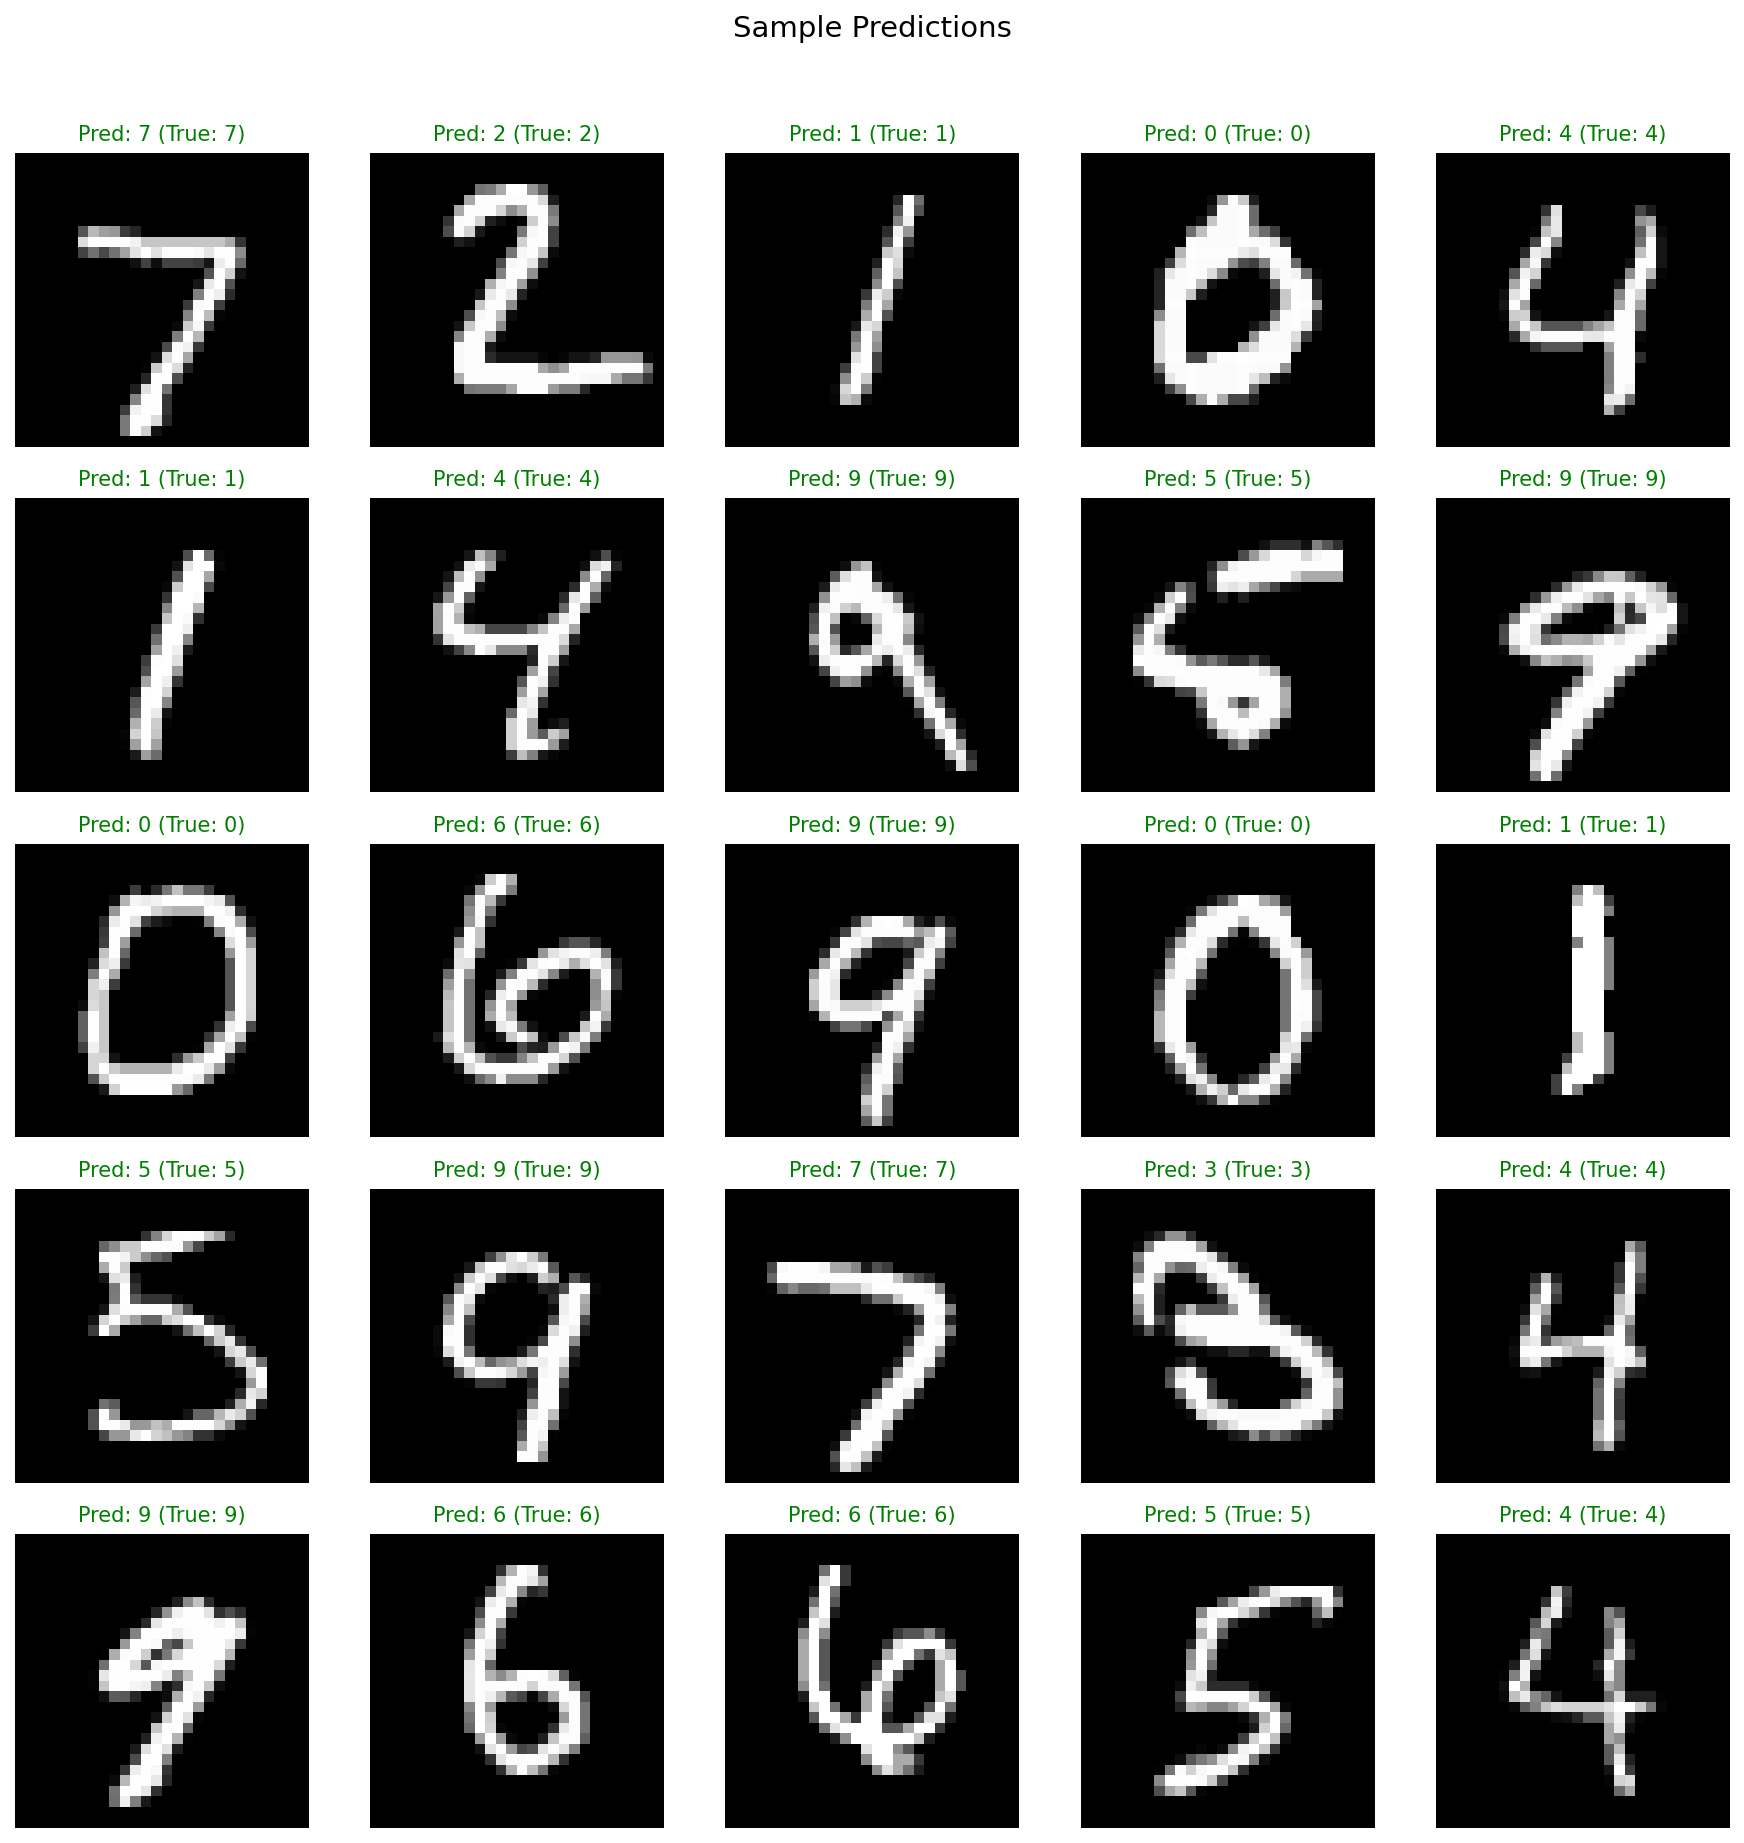
\includegraphics[width=0.9\textwidth]{figures/mnist_predictions.png}
    \caption{Sample predictions on test images}
    \label{fig:mnist_predictions}
\end{figure}

\begin{table}[H]
\centering
\caption{Handwritten Digit Recognition Model Performance}
\begin{tabular}{lc}
\toprule
\textbf{Metric} & \textbf{Value} \\
\midrule
Test Accuracy & 98.7\% \\
Model Size (Float32) & 245 KB \\
Model Size (Int8 Quantized) & 72 KB \\
Inference Time (STM32F4) & $\sim$15 ms \\
\bottomrule
\end{tabular}
\end{table}

\subsection{TensorFlow Lite Conversion}

Similar to the keyword spotting model, we apply full integer quantization:

\begin{lstlisting}[language=Python, caption=TFLite Conversion for MNIST Model]
def representative_dataset():
    for i in range(1000):
        yield [x_train[i:i+1].astype(np.float32)]

converter = tf.lite.TFLiteConverter.from_keras_model(model)
converter.optimizations = [tf.lite.Optimize.DEFAULT]
converter.representative_dataset = representative_dataset
converter.target_spec.supported_ops = [
    tf.lite.OpsSet.TFLITE_BUILTINS_INT8
]
converter.inference_input_type = tf.int8
converter.inference_output_type = tf.int8
tflite_model = converter.convert()
\end{lstlisting}

\subsection{STM32 Deployment}

The deployment process involves:

\begin{itemize}
    \item Converting TFLite model to C array using \texttt{xxd}
    \item Configuring TensorFlow Lite Micro runtime
    \item Implementing image capture interface
    \item Processing and displaying results via UART/LCD
\end{itemize}

%==============================================================================
\section{Comparison and Discussion}
%==============================================================================

\begin{table}[H]
\centering
\caption{Comparison of Both Applications}
\begin{tabular}{lcc}
\toprule
\textbf{Aspect} & \textbf{Keyword Spotting} & \textbf{Digit Recognition} \\
\midrule
Input Type & Audio (1D temporal) & Image (2D spatial) \\
Feature Extraction & Spectrogram & None (raw pixels) \\
Model Size (Quantized) & 365 KB & 72 KB \\
Test Accuracy & 89.0\% & 98.7\% \\
Inference Time & $\sim$50 ms & $\sim$15 ms \\
Complexity & Higher & Lower \\
\bottomrule
\end{tabular}
\end{table}

\subsection{Key Observations}

\begin{enumerate}
    \item The digit recognition model achieves higher accuracy with a smaller model size, primarily due to the simpler nature of the classification task.
    
    \item Keyword spotting requires more complex feature extraction (MFCC), which adds to the overall processing time.
    
    \item Both models fit comfortably within the memory constraints of STM32F4 series microcontrollers.
    
    \item Quantization provides approximately 4× reduction in model size with minimal accuracy loss.
\end{enumerate}

%==============================================================================
\section{Conclusion}
%==============================================================================

This homework successfully demonstrated the implementation of two embedded machine learning applications on STM32 microcontrollers. Both the keyword spotting and handwritten digit recognition systems achieve high accuracy while meeting the resource constraints of embedded systems.

Key takeaways include:
\begin{itemize}
    \item Careful model architecture design is crucial for embedded deployment
    \item Quantization is essential for reducing model size without significant accuracy loss
    \item Feature extraction (like MFCC) can be performed on-device for real-time applications
    \item TensorFlow Lite for Microcontrollers provides a practical framework for embedded ML
\end{itemize}

The complete source code and trained models are available in the GitHub repository.

%==============================================================================
\section*{References}
%==============================================================================

\begin{thebibliography}{9}

\bibitem{unsalan2025}
C. Ünsalan, B. Höke, and E. Atmaca, \textit{Embedded Machine Learning with Microcontrollers: Applications on STM32 Boards}, Springer Nature, ISBN: 978-3031709111, 2025.

\bibitem{speechcommands}
P. Warden, "Speech Commands: A Dataset for Limited-Vocabulary Speech Recognition," arXiv preprint arXiv:1804.03209, 2018.

\bibitem{mnist}
Y. LeCun, C. Cortes, and C.J.C. Burges, "The MNIST Database of Handwritten Digits," 1998.

\bibitem{tflite}
TensorFlow Team, "TensorFlow Lite for Microcontrollers," \url{https://www.tensorflow.org/lite/microcontrollers}.

\end{thebibliography}

\end{document}

